Cette préface est destinée à tous les lecteurs, toutes les lectrices, et pas
seulement les mathématiciens et mathématiciennes. Après les remerciements
d'usage, on présentera quelques applications des \emph{corps finis}, l'objet au
cœur de ce document, afin de comprendre l'étendue de leur utilité. Celles et ceux
voulant assouvir leur soif de détails techniques et de mathématiques
pourront le faire en parcourant les références bibliographiques proposées. Cela
sera sans doute aussi possible (jusqu'à un certain point) en lisant les autres
chapitres de ce manuscrit, ainsi que la fin de cette préface, qui donne un
résumé détaillé du contenu du document.

\minitoc
% TODO
% ====
%
% Find an illustration (something linked with crypto preferably)
\clearpage

\section*{Remerciements}
\addcontentsline{toc}{section}{Remerciements}

\clearpage
\section*{Applications des corps finis}
\addcontentsline{toc}{section}{Applications des corps finis}

On peut se demander, probablement à juste titre, à quoi sert une thèse en
mathématiques fondamentales. J'ai la chance d'avoir travaillé sur un sujet qui,
quoique relativement abstrait, possède des applications extrêmement utiles, et
ce dans la vie de tous les jours, pour quasiment tout le monde. Nous allons donc
voir deux applications élégantes des \emph{corps finis}, qui illustrent
l'intérêt de ces objets mathématiques.

\subsection*{Cryptographie}
\addcontentsline{toc}{subsection}{Cryptographie}
\label{sec:crypto}

Pendant toute la durée de mon doctorat, j'ai expliqué aux non-mathématiciens que
je faisais une thèse en \emph{cryptographie}. C'est en fait un mensonge, car
même si le titre initial du projet de thèse était \emph{Arithmétique efficace
pour la cryptographie et la cryptanalyse}, je me suis finalement intéressé
aux deux premiers mots seulement : arithmétique efficace. Cependant, la
cryptographie reste une source d'inspiration et une des motivations derrière ces
travaux. Les recherches que nous avons menées viennent souvent de la
cryptographie, ou bien ont une application dans cette discipline, nous
commencerons donc par expliquer ce que ``cryptographie'' signifie.

Nous sommes des animaux sociaux, et nous avons donc besoin de communiquer les
uns avec les autres. Parfois, nous voulons que nos échanges restent privés.
Les raisons derrière ce souhait peuvent être multiples : informations
militaires, commerciales, médicales, bancaires, histoires amoureuses... La
cryptographie est la science qui étudie les techniques utilisées pour sécuriser
les communications, en présence d'une tierce partie appelée \emph{adversaire}.
Historiquement, la cryptographie s'est d'abord concentrée sur le chiffrement des
messages (leur confidentialité), c'est-à-dire rendre le message illisible pour
quelqu'un qui l'intercepterait ou en obtiendrait une copie. Pour que le
destinataire légitime du message puisse le lire, il faut alors le
\emph{déchiffrer}. C'était uniquement possible lorsqu'à la fois l'émetteur du
message et son destinataire partagaient un secret commun au préalable, secret
qui était alors utilisé aussi bien pour chiffrer que pour déchiffrer le message.
Dans un protocole cryptographique, le secret commun est appelé une
\emph{clé}, parce que le chiffrement est vu comme un cadenas. Cette méthode de
chiffrement est appelée chiffrement symétrique car les deux participants
partagent le même secret. La situation est résumée sur la
Figure~\ref{fig:crypto-sym}.
\begin{figure}
  \centering
  \begin{tikzpicture}
    \node (msg) at (0,0) {Message};
    \node (msg-enc) at (6,0) {Message chiffré};
    \node (msg-rec) at (12,0) {Message};
    \node (secret) at (6, 2) {Secret};
    \node (enc) at (2.15,1.8) {Chiffrement};
    \node (dec) at (9.75,1.8) {Déchiffrement};

    \draw[->] (msg) -- (msg-enc);
    \draw[->] (msg-enc) -- (msg-rec);
    \draw[->] (secret) to[bend right] (2.2,0);
    \draw[->] (secret) to[bend left] (9.8,0);
    \node (a) at (2.2,1) {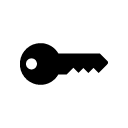
\includegraphics[scale=0.3]{img/key-128.png}};  
    \node (b) at (9.8,1) {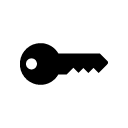
\includegraphics[scale=0.3]{img/key-128.png}};  
    \node (c) at (6,-1) {
\includegraphics[scale=0.05]{img/lock-128.png}};  
  \end{tikzpicture}
  \caption{La stratégie générale d'un protocole de chiffrement symétrique.}
  \label{fig:crypto-sym}
\end{figure}
Le chiffre de César est un vieil exemple de protocole cryptographique, dans lequel
chaque lettre du message est remplacée par une autre lettre. Toutes les lettres
sont décalées par un nombre constant $n$ de positions vers le début de
l'alphabet. Par exemple, avec $n=3$, la lettre \texttt{D} devient \texttt{A}, la
lettre \texttt{E} devient \texttt{B}, la lettre \texttt{F} devient
\texttt{C}, et ainsi de suite. Ce protocole doit son nom à Jules César, qui
l'utilisait pour communiquer avec sa famille, avec un décalage de $n=3$. Dans la
Figure~\ref{fig:caesar}, on a dessiné un schéma représentant la correspondance
entre les lettres avec le décalage $n=3$. L'anneau extérieur représente les
lettres dans le texte brut (le texte original, sans chiffrement), tandis que
l'anneau intérieur correspond aux lettres dans le texte chiffré.
\begin{figure}
  \centering
  \begin{tikzpicture}[x=1em,y=1em]
%   set up
    \pgfmathsetmacro\angdiv{360/26}
    \pgfmathtruncatemacro\caeser{3} % Input Caeser shift here! (positive for clockwise)
    \coordinate (n-0) at (90+\angdiv/2:7) {};
    \coordinate (m-0) at (90-\caeser*\angdiv+\angdiv/2:5) {};
%   draw Caeser diagram
    \draw circle [radius=8] circle [radius=6.5] circle [radius=6]  circle [radius=4.5]
        \foreach \i in {0,...,25}{%
            ($({90-(\i-1/2)*\angdiv}:8)$) -- ($(({90-(\i-1/2)*\angdiv}:6.5)$)
            ($({90-(\i-1/2)*\angdiv}:4.5)$) -- ($(({90-(\i-1/2)*\angdiv}:6)$)
        };
    \foreach [count=\a from 0] \text in {A,B,...,Z}{
        \pgfmathtruncatemacro\b{\a+1}%
        \path [curved text=\text] (n-\a) arc [start angle=90-(\a-1/2)*\angdiv, delta angle=-\angdiv, radius=7] node (n-\b) {};
        \path [curved text=\text] (m-\a) arc [start angle=90-(\a+\caeser-1/2)*\angdiv, delta angle=-\angdiv, radius=5] node (m-\b) {}; % Inner circle
    }
%   draw arrow
    \draw [-latex, thick] (65:9.5) to[bend left=20,edge label=$+3$] (40:9.5);
    \end{tikzpicture}
  \caption{Representation du chiffre de César avec le décalage $n=3$.}
  \label{fig:caesar}
\end{figure}
Dans cet exemple, la clé secrète du protocole est la valeur $n$ du décalage :
connaissant $n$, on peut à la fois chiffrer et déchiffrer des messages. Le
chiffre de César est suffisamment simple pour être exécuté par une machine, mais
il n'est plus utilisé aujourd'hui. En effet, le faible nombre de clés possibles
lorsque ce protocole est utilisé est petit, et un adversaire (un espion, un
ennemi...) peut donc facilement deviner le message brut en essayant toutes les
clés possibles. On pourrait même demander à un ordinateur de faire cette
recherche, ce qui accélèrerait encore les choses. C'est pourquoi, en
cryptographie moderne, le nombre de clés utilisables doit être bien plus grand.
Par exemple, le protocole standard de chiffrement symétrique, appelé AES (pour
Advanced Encryption Standard), a été créé en 1999~\cite{DR99, DR02} et peut être
utilisé avec $2^{128}$, $2^{192}$, ou $2^{256}$ clés différentes, en fonction de
la version de chiffrement utilisée. Le plus petit de ces nombres peut aussi
s'écrire
\[
  2^{128} = 340282366920938463463374607431768211456,
\]
alors qu'un milliard s'écrit
\[
  10^{9} = 1000000000,
\]
ce sont donc des nombres vraiment très grands.

Le nombre de clés possibles n'est pas la seule chose ayant changé depuis Jules
César.
D'abord, les communications sont désormais essentiellement numériques, et donc
la cryptographie fait partie de l'informatique. C'est très important parce que
cela signifie que les travaux réalisés pendant cette thèse sont aussi orientés
vers l'informatique : on souhaite obtenir des résultats mathématiques qui sont
\emph{effectifs}, c'est-à-dire qui sont utilisables par un ordinateur. Ensuite,
l'étendue de la cryptographie est aujourd'hui bien plus large. Dans la
cryptographie moderne, le chiffrement symétrique ne constitue qu'un seul domaine
de la cryptographie, qui possède bien d'autres aspects, comme le chiffrement
asymétrique (aussi appelé chiffrement à clé publique), l'intégrité des données,
l'authentification, les signatures numériques (la liste n'est pas exhaustive).
Nous n'expliquerons pas tous ces termes, mais les personnes intéressées peuvent
lire les introductions sur chacun de ces sujets dans~\cite{MVOV18}, par exemple.
Un changement majeur en cryptographie a eu lieu en 1976, avec l'article pionnier
\emph{New Directions in Cryptography}~\cite{DH76} de Diffie et Hellman, qui ont
inventé ce qu'on appelle la cryptographie à clé publique. On présente brièvement
la cryptographie à clé publique, afin de la comparer avec la cryptographie
symétrique.

Un des désavantages principaux du chiffrement symétrique est que les deux
personnes participantes doivent détenir un secret en commun afin de pouvoir
communiquer de manière sécurisée. On peut imaginer qu'elles se donnent
rendez-vous en personne pour se mettre d'accord sur un secret, mais cela n'est
pas toujours possible, par exemple si elles vivent très loin l'une de l'autre.
Elles pourraient alors trouver un autre moyen de communication pour s'échanger
leur secret, mais ce moyen de communication ne serait pas sécurisé justement
parce qu'elles n'ont pas encore pu échanger de secret. On a ainsi l'impression
qu'on se mord la queue et que le problème est insoluble. En fait, le chiffrement
à clé publique vient justement résoudre ce problème, car il permet de chiffrer
des messages sans avoir connaissance d'un secret commun. L'idée très élégante de
Diffie et Hellman est de casser la symétrie entre les personnes participantes
(qu'on appellera Alice et Bob, car c'est la tradition en cryptographie).
Au lieu de se mettre d'accord sur un secret commun, seul l'un des participants
(par exemple Alice) crée une \emph{paire} de clés : l'une d'elle va être
publique et est destinée à être transmise à tout le monde, alors que l'autre est
privée et doit être connue d'Alice seulement. Avec la clé publique, chacun peut
chiffrer un message, alors que la clé privée est nécessaire quant à elle au
déchiffrement. En utilisant ce genre de système, tout le monde peut envoyer un
message chiffré à Alice, car la clé à utiliser pour cela est publique, mais
seule Alice peut déchiffrer ces messages, même s'ils sont interceptés par un
éventuel adversaire. Ainsi les communications restent sécurisées. Nous donnons un
schéma du fonctionnement général du chiffrement à clé publique dans la
Figure~\ref{fig:crypto-asym}.
\begin{figure}
  \centering
  \begin{tikzpicture}
    \node (msg) at (0,0) {Message};
    \node (msg-enc) at (6,0) {Message chiffré};
    \node (msg-dec) at (12,0) {Message déchiffré};
    \node (bob) at (0,2) {Bob};
    \node (alice) at (12, 2) {Alice};
    \node (key-pub) at (5, 2) {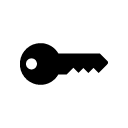
\includegraphics[scale=0.3]{img/key-128.png}};
    \node (key-pub-txt) at (4.8, 3) {Clé publique};
    \node (key-pri) at (7, 2) {
\includegraphics[scale=0.065]{img/key-512.png}};
    \node (key-pri-txt) at (6.9, 3) {Clé privée};
    \node (lock) at (6,-1) {
\includegraphics[scale=0.05]{img/lock-128.png}};  
    \draw[->] (msg) -- (msg-enc);
    \draw[->] (msg-enc) -- (msg-dec);
    \draw[->] (bob) to[bend left, edge label=Chiffre] (2.5,0);
    \node (key-pub2) at (2.2, .8) {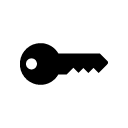
\includegraphics[scale=0.3]{img/key-128.png}};
    \draw[->] (alice) to[bend right, edge label = Déchiffre] (9,0);
    \node (key-pri2) at (9.4, .8) {
\includegraphics[scale=0.065]{img/key-512.png}};
    \draw[->] (alice) to (8,2);
    \node (c) at (9.5, 2.3) {Crée};
  \end{tikzpicture}
  \caption{Idée générale du chiffrement à clé publique.}
  \label{fig:crypto-asym}
\end{figure}
Avec un tel système, Bob ne peut pas recevoir de message, il peut uniquement en
envoyer à Alice. Si Alice veut envoyer un message à Bob en utilisant du
chiffrement à clé publique, Bob doit alors créer sa propre paire de clé. Il
donne alors sa clé publique à Alice, qui peut l'utiliser pour chiffrer un
message et l'envoyer à Bob. Bob déchiffre alors le message en utilisant sa clé
privée. La cryptographie à clé publique est plus lourde à mettre en place que la
cryptographie symétrique, une autre solution est donc pour Bob de choisir un
secret, de le chiffrer, puis de l'envoyer à Alice, qui pourra le déchiffrer et
ils pourront alors tous les deux l'utiliser pour mettre en place un protocole de
chiffrement symétrique. C'est ce qui est fait en pratique : seul un
\emph{échange de clé} a lieu en utilisant la cryptographie à clé publique, le
reste étant géré par la cryptographie symétrique. Néanmoins, la cryptographie à
clé publique est fondamentale car elle permet la mise en place de la
cryptographie symétrique.

Le premier protocole d'échange de clé a été inventé par Diffie et Hellman en
1976~\cite{DH76}, et un exemple de chiffrement à clé publique est donné par
Rivest, Shamir et Adleman avec le protocole RSA~\cite{RSA78} qu'ils ont décrit en
1977. Ces deux protocoles sont tous les deux basés sur des structures
mathématiques. En effet, les mathématiques sont un moyen pratique d'étudier et
d'expliquer la cryptographie, par exemple le chiffre de César avec le décalage
$n=3$
peut être expliqué en représentant les lettres par des nombres entre $0$ et $25$
\[
  \texttt{A}\to 0, \texttt{B} \to 1, \dots,\texttt{Y}\to24, \texttt{Z}\to25
\]
et en définissant le chiffrement par la soustraction par $3$. Avec cette
représentation, on admet que le nombre $-1$ est équivalent au nombre
$25$, c'est-à-dire qu'avant le \texttt{A} vient la lettre \texttt{Z}, que le
nombre $-2$ est équivalent au nombre $24$, c'est-à-dire que deux lettres avant
le \texttt{A} vient la lettre \texttt{Y}, et ainsi de suite. En fait, une partie
des mathématiques appelée \emph{théorie des nombres} est dédiée à l'étude de ce
genre de nombres joints à des règles comme celle que nous venons d'énoncer :
$-1=25$. Ces ensembles de nombres sont appelés des \emph{groupes cycliques}, car
ils peuvent être représentés par un cercle. Celui que nous avons évoqué est noté
\[
  \mathbb{Z}/26\mathbb{Z}
\]
et peut être représenté par la Figure~\ref{fig:cyclic-group}.
\begin{figure}
  \centering
  \begin{tikzpicture}
    \foreach \x in {0, 1,...,25} \coordinate (\x) at (13.85*\x:3);
    \draw[additive-structure] (0,0) circle (3);
    \foreach \x in {0, 1,...,25} \draw[fill] (13.85*\x:3) circle (.1);
    \foreach \x in {0, 1,...,25} \node (p) at (13.85*\x:3.4) {$\x$};
  \end{tikzpicture}
  \caption{Le groupe cyclique $\mathbb{Z}/26\mathbb{Z}$ représenté par un
cercle.}
  \label{fig:cyclic-group}
\end{figure}
De nombreuses autres structures intéressantes existent, on peut
lire~\cite{Lang04, Perrin96} pour en apprendre plus à leur sujet ou pour
découvrir les richesses de l'algèbre. Avec le développement de la cryptographie
à clé publique, la théorie des nombres en est devenue la pierre angulaire, et
des concepts mathématiques plus élaborés ont été utilisés, comme les corps
finis, les courbes elliptiques, ou les isogénies. Sans entrer dans les détails,
ce qui est important est que la sécurité des protocoles cryptographiques est
basée sur des problèmes mathématiques difficiles faisant intervenir ces
concepts. Ainsi, une meilleure compréhension de ces objets implique une
meilleure compréhension de la sécurité de nos protocoles cryptographiques. La
partie de la cryptographie dont le rôle est d'analyser la sécurité de ces
protocoles (c'est-à-dire, de les ``casser'') est appelée la \emph{cryptanalyse}.

En outre, puisque les protocoles sont basés sur des manipulations dans ces
objets, une meilleure compréhension de ces derniers implique également de
meilleurs (en particulier, plus rapides) protocoles cryptographiques. Comme la
cryptographie est omniprésente dans les communications modernes (sur Internet,
quand vous utilisez votre carte de crédit, sur les applications de messagerie de
votre téléphone, ...), avoir des protocoles efficaces est crucial. Il est donc
nécessaire d'être capable de manipuler efficacement les concepts mathématiques
qui se cachent derrière nos protocoles, que ce soit pour la cryptographie
(mettre en place des protocoles performants) ou la cryptanalyse (analyser leur
sécurité). Par ``manipuler'', on entend être capable de faire des additions, des
multiplications, et parfois des opérations plus compliquées avec ces objets. La
science qui étudie comment faire tout cela s'appelle \emph{l'arithmétique}. En
conclusion, il est nécessaire d'avoir une arithmétique efficace pour la
cryptographie et la cryptanalyse.

\subsection*{Théorie des codes}
\addcontentsline{toc}{subsection}{Théorie des codes}
\label{sec:coding}

Une autre application élégante (et utile) des corps finis est la \emph{théorie
des codes}. Comme la cryptographie, la théorie des codes est liée aux
communications, mais elle répond à un problème complètement différent. Nous
faisons maintenant l'hypothèse qu'Alice et Bob veulent communiquer, et que les
informations qu'ils veulent échanger vont traverser un canal de communication.
En pratique, ce canal peut être de la fibre optique, des fils électriques, des
ondes radio, et beaucoup d'autres choses encore. On suppose qu'Alice veut
envoyer le message ``Salut ! Ça va ?'' à Bob. En réalité, ces lettres vont
probablement d'abord être transformées en une suite de bits : \texttt{0} et
\texttt{1}, on imaginera donc qu'Alice envoit le message
\[
  m = \texttt{0010110001010111}
\]
à travers le canal. Souvent, dans des conditions réelles, le canal de
communication est imparfait, et est sujet à du \emph{bruit}, c'est-à-dire qu'à
cause de la qualité du canal, ou à cause de l'environnement, des erreurs peuvent
apparaître et changer le message envoyé par Alice, comme montré sur la
Figure~\ref{fig:communication-channel}.
\begin{figure}
  \centering
  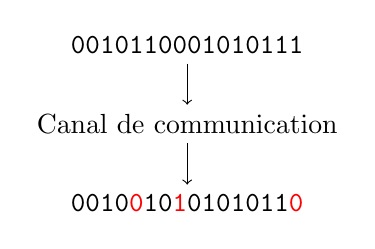
\begin{tikzpicture}
    \node (msg) at (0,2) {\texttt{0010110001010111}};
    \node (msg-dec) at (0,0)
    {\texttt{0010\textcolor{red}{0}10\textcolor{red}{1}0101011\textcolor{red}{0}}};
    \node (channel) at (0, 1) {Canal de communication};
    \draw[->] (msg) -- (channel);
    \draw[->] (channel) -- (msg-dec);
  \end{tikzpicture}
  \caption{Un canal de communication imparfait.}
  \label{fig:communication-channel}
\end{figure}
Sans autre outil ou contexte, il peut être difficile (voire impossible) pour Bob
de deviner ce que voulait dire Alice. La théorie des codes étudie les moyens de
lutter contre l'apparition d'erreurs et de retrouver le message initial, même
une fois modifié. Le but est de construire ce qu'on appelle des \emph{codes} qui
vont être capable de corriger des erreurs, on les nommera donc \emph{codes
correcteurs d'erreurs}. L'idée est que pour être sûr qu'une information, qui est
représentée par un \texttt{0} ou un \texttt{1}, arrive jusqu'à Bob sans erreur,
Alice va la répéter plusieurs fois. Par exemple, si Alice répète chaque bit
trois fois, en faisant des mots de trois symboles :
\[
  \texttt{0}\to\texttt{000}\quad\quad\texttt{1}\to\texttt{111},
\]
alors une erreur peut être corrigée, car si Bob reçoit, par exemple, le mot
\texttt{001}, il sait qu'il s'agit probablement du mot \texttt{000} qui a subit
une erreur de transmission. Il peut alors interpréter le mot \texttt{001} comme
venant du bit initial \texttt{0} dans le message d'Alice. Plus généralement, si
Bob reçoit un mot \texttt{abc}, il l'interprétera comme venant du bit
\texttt{0} s'il y a une majorité de \texttt{0} dans le mot \texttt{abc}.
Réciproquement, s'il y a une majorité de \texttt{1} dans le mot
\texttt{abc}, il l'interprétera comme venant du bit \texttt{1}. Bien entendu,
s'il y a trop d'erreurs de transmission dans un seul mot, il est possible de mal
interpréter le message. Par exemple, si le mot \texttt{000} devient
\texttt{110} après être passé dans le canal de communication, alors Bob
le décodera comme $\texttt{111}\to\texttt{1}$. Cette stratégie est connue sous
le nom de code de répétition de longueur $3$, et est un exemple de code
correcteur d'erreur. La procédure complète est décrite dans la
Figure~\ref{fig:rep3}.
\begin{figure}
  \centering
  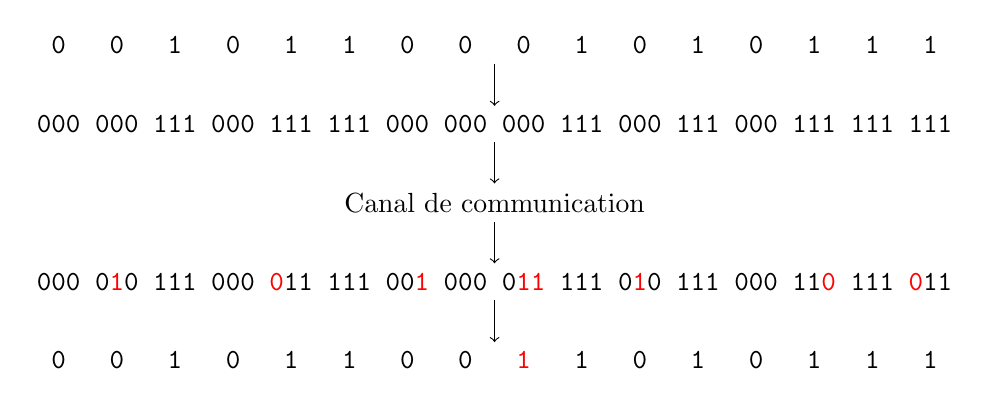
\begin{tikzpicture}
    \node (msg-init) at (0,3)
    {\texttt{\phantom{ }0\phantom{ } \phantom{ }0\phantom{ } \phantom{
    }1\phantom{ }  \phantom{ }0\phantom{ }  \phantom{ }1\phantom{ }  \phantom{
    }1\phantom{ }  \phantom{ }0\phantom{ }  \phantom{ }0\phantom{ }  \phantom{
    }0\phantom{ }  \phantom{ }1\phantom{ }  \phantom{ }0\phantom{ }  \phantom{
    }1\phantom{ }  \phantom{ }0\phantom{ }  \phantom{ }1\phantom{ }  \phantom{
    }1\phantom{ }  \phantom{ }1\phantom{ }}};
    \node (msg) at (0,2)
    {\texttt{000 000 111 000 111 111 000 000 000 111 000 111 000 111 111 111}};
    \node (msg-dec) at (0,0)
  {\texttt{000 0\textcolor{red}{1}0 111 000 \textcolor{red}{0}11 111
  00\textcolor{red}{1} 000 0\textcolor{red}{11} 111 0\textcolor{red}{1}0 111 000 11\textcolor{red}{0} 111 \textcolor{red}{0}11}};
    \node (channel) at (0, 1) {Canal de communication};
    \node (msg-end) at (0,-1)
    {\texttt{\phantom{ }0\phantom{ } \phantom{ }0\phantom{ } \phantom{
    }1\phantom{ }  \phantom{ }0\phantom{ }  \phantom{ }1\phantom{ }  \phantom{
    }1\phantom{ }  \phantom{ }0\phantom{ }  \phantom{ }0\phantom{ }  \phantom{
    }\textcolor{red}{1}\phantom{ }  \phantom{ }1\phantom{ }  \phantom{ }0\phantom{ }  \phantom{
    }1\phantom{ }  \phantom{ }0\phantom{ }  \phantom{ }1\phantom{ }  \phantom{
    }1\phantom{ }  \phantom{ }1\phantom{ }}};
    \draw[->] (msg-init) -- (msg);
    \draw[->] (msg) -- (channel);
    \draw[->] (channel) -- (msg-dec);
    \draw[->] (msg-dec) -- (msg-end);
  \end{tikzpicture}
  \caption{Le code de répétition de longueur $3$.}
  \label{fig:rep3}
\end{figure}
Afin de corriger plus d'erreurs, on pourrait utiliser des codes de répétition
avec des longueurs plus grandes. Néanmoins, lorsqu'on utilise un code de
répétition de longueur $n$, il faut envoyer $n$ fois plus d'information à
travers le canal, ce qui peut avoir un prix dans des situations réelles. Il faut
donc trouver un équilibre entre le surcoût induit par la longueur du code et le
nombre d'erreurs que l'on souhaite être capable de corriger. En fait, en
fonction de la qualité du canal de communication, tous les codes ne conviennent
pas. Claude Shannon a prouvé en 1948~\cite{Shannon48} que l'on peut définir une
quantité appelé \emph{capacité} du canal qui mesure essentiellement la quantité
d'information que l'on peut faire passer à travers un canal. Cela mesure aussi
combien de répétitions on doit inclure dans notre code pour que le message soit
transmis de manière fiable. La théorie des codes est un domaine de recherche
actif, et il n'existe donc pas de réponse définitive à la question ``Quel est le
meilleur code que nous pouvons utiliser ?''. Les codes utilisés en pratique sont
un peu plus subtils que le code de répétition, mais ils suivent la même logique.
Par exemple, les codes de Reed-Solomon~\cite{RS60}, utilisés dans des
technologies de la vie de tous les jours comme les CDs, les DVDs, les disques
Blu-ray, ou encore dans les missions de la NASA, font intervenir des mots
composés de suites de valeurs prises dans un corps fini. D'autres codes, comme
les codes de Goppa géométriques~\cite{Goppa81}, sont basés sur les corps de
fonctions algébriques, une structure mathématique qui est construite à partir
des corps finis. En conclusion, exactement comme en cryptographie, les corps
finis sont omniprésents en théorie des codes, et une arithmétique efficace dans
les corps finis permet à la fois un codage et un décodage performant.

\section*{Arithmétique des corps finis}
\addcontentsline{toc}{section}{Arithmétique des corps finis}

Comme énoncé dans les pages précédentes, les protocoles cryptographiques et les
codes sont basés sur des structures mathématiques pour fonctionner. Celle que
nous étudions tout au long de ce document est appelée \emph{corps fini}. Un
\emph{corps} est une structure mathématique (on dit aussi \emph{structure
algébrique}) composée d'éléments que l'on peut additionner, soustraire,
multiplier, et diviser (excepté par zéro). C'est une structure bien connue :
l'ensemble des nombres réels, noté $\mathbb{R}$, en est un exemple. En effet,
les éléments de $\mathbb{R}$, par exemple $0$, $1$, $-3,5631$, mais aussi des
nombres plus compliqués comme $\pi$, $\sqrt2$, ou $\frac{7}{13}$ peuvent être
additionnés, soustraits, multipliés, ou divisés. Les nombres dans $\mathbb{R}$
peuvent avoir une infinité de décimales, par exemple les $60$ premières
décimales de la constante $\pi$ sont
\[
  \pi = 3.14159265358979323846264338327950288419716939937510582097494\dots.
\]
Un ordinateur n'a qu'une mémoire finie, c'est-à-dire que la quantité
d'information qu'il peut stocker n'est pas illimitée. Par conséquent, il est
impossible de stocker toutes les décimales de $\pi$, et, plus généralement, les
décimales de beaucoup d'autres nombres de $\mathbb{R}$, sur un ordinateur. Cela
reste possible de travailler avec des nombres dans $\mathbb{R}$ sur un
ordinateur, mais il est plus simple de manipuler des éléments
qui viennent d'une structure algébrique \emph{finie}, c'est-à-dire composée d'un
nombre $n$ d'éléments, avec 
\[
  n < \infty.
\]
Un exemple de ce type de structure a déjà été donné : le groupe cyclique
$\mathbb{Z}/26\mathbb{Z}$ qui est composé des ``nombres'' $0, 1, \dots, 25$.
Cependant, ce ne sont pas les mêmes nombres que ceux que nous connaissons, car
avec les éléments de $\mathbb{Z}/26\mathbb{Z}$, on a par exemple l'égalité
\[
  3-4 = -1 = 25,
\]
ce qui n'est pas correct pour les vrais nombres dans $\mathbb{R}$, mais nous
écrivons tout de même les nombres de $\mathbb{Z}/26\mathbb{Z}$ comme ceux de
$\mathbb{R}$ par simplicité. Nous avons déjà défini une addition et une
soustration dans $\mathbb{Z}/26\mathbb{Z}$, et nous pourrions aussi définir une
multiplication et une division d'une manière naturelle. Les corps finis sont une
généralisation des espaces comme $\mathbb{Z}/26\mathbb{Z}$. Bien que l'ensemble
$\mathbb{Z}/26\mathbb{Z}$ ne soit pas un corps, pour des raisons techniques,
cela reste une bonne approximation, pour cette introduction en tous cas, de
penser les corps finis comme ce genre d'ensemble.

Comme les éléments d'un corps fini sont, par définition, en nombre fini, c'est
relativement plus facile de les manipuler avec un ordinateur. De plus, la
structure de corps nous permet de manipuler les éléments des corps finis comme
des nombres classiques (c'est-à-dire avec des additions, multiplications, ...),
ce qui les rend utiles. C'est pourquoi aujourd'hui, les corps finis sont
absolument partout dans des domaines comme la cryptographie ou la théorie des
codes.

Parfois, certains problèmes mathématiques simples sont bien compris d'un point
de vue théorique, mais il existe toujours des questions ouvertes concernant
certains aspects pratiques. Par exemple, la multiplication de deux entiers $a$
et $b$ de $\mathbb{N}$ est un problème simple, qui peut être fait à la main par
des enfants. Pourtant, la façon optimale de multiplier deux entiers
gr\^ace à un ordinateur reste un problème ouvert, pour lequel des articles de
recherche sont régulièrement publiés~\cite{HVDH19}. L'arithmétique des corps
finis, c'est-à-dire comment faire des opérations comme l'addition ou la
multiplication, est très bien comprise, car la structure des corps finis est
assez simple. Pour autant, la meilleure façon de multiplier deux éléments dans
un corps fini est également inconnue. C'est exactement le sujet de cette thèse :
l'étude de l'arithmétique des corps finis.

\section*{Résumé des travaux}
\addcontentsline{toc}{section}{Résumé des travaux}

Ce résumé présente de manière détaillée l'ensemble des travaux réalisés pendant
ma thèse, ainsi que la façon dont est organisé ce manuscrit. Cette partie est
donc dédiée à un ``public scientifique averti''.

\subsection*{Arithmétique efficace dans une extension fixée}
\addcontentsline{toc}{subsection}{Arithmétique efficace dans une extension fixée}

Ce document est composé de deux parties, qui sont essentiellement indépendantes.
Dans la Partie~\ref{part:single}, nous étudions l'arithmétique d'une extension
de corps fini fixée
\[
  \mathbb{F}_{p^{k}}.
\]
\paragraph{Préliminaires.} Nous commençons dans le
Chapitre~\ref{chap:preliminary} par rappeler les faits fondamentaux concernant
les objets que nous utiliserons dans le reste du document. En particulier, on
rappelle la structure des corps finis, ainsi que la manière de les construire
comme des quotients d'anneaux de polynômes
\[
  \mathbb{F}_p[x]/(P(x)).
\]
Nous donnons quelques propriétés des extensions de corps finis concernant leur
structure d'espace vectoriel ainsi que sur leur groupe d'automorphismes.

Dans la Section~\ref{sec:algebraic-function-fields}, nous présentons les
\emph{corps de
fonctions algébriques}, une structure algébrique que nous utilisons dans les
preuves des Chapitres~\ref{chap:bilinear} et~\ref{chap:hypersymmetric}. On
rappelle brièvement ce que sont les \emph{places}, et qu'elles sont
essentiellement équivalentes aux notions de valuations discrètes et d'anneaux de
valuations. On décrit comment évaluer un élément $z$ d'un corps de fonction
algébrique à une place $P$, et on donne la définition d'un zéro et d'un pôle, ce
qui justifie le nom de corps de ``fonction''. Enfin, on donne la définition d'un
\emph{diviseur} et on rappelle les résultats habituels de la théorie : le lien
entre le degré et la dimension d'un diviseur, la définition du \emph{genre} d'un
corps de fonctions algébrique, et le théorème de Riemann-Roch.

Dans la Section~\ref{sec:complexity-models}, on donne le modèle de la
\emph{complexité algébrique} et on explique pourquoi ce modèle est pertinent
pour nos travaux. On rappelle également les notions de \emph{grand O} et
\emph{petit o}, qui sont utilisées pour exprimer des résultats asymptotiques.

Enfin, dans la Section~\ref{sec:fundamental-algos}, nous donnons des références
bibliographiques, ainsi que la complexité de certains algorithmes classiques et
importants dans notre travail : l'algorithme de Brent-Kung pour la composition
modulaire, le calcul de polynôme minimal, et l'algorithme de Berlekamp-Massey.
Ces routines sont utilisées dans plusieurs algorithmes de ce manuscrit, notamment
dans les Chapitres~\ref{chap:isomorphism} et~\ref{chap:standard}.

\paragraph{Complexité bilinéaire et algorithmes de type Chudnovsky$^2$.} Dans le
Chapitre~\ref{chap:bilinear}, nous présentons la théorie de la \emph{complexité
bilinéaire}, un modèle alternatif de complexité utilisé pour mesurer le coût de
calcul de certaines applications bilinéaires. Dans ce modèle, seules les
multiplications sont comptées, ce qui est justifié par le fait qu'en pratique
les multiplications sont plus coûteuses que les additions. La complexité
bilinéaire d'une application est alors donnée par le nombre minimal de
multiplications nécessaires au calcul de l'application en question. L'algorithme
de Karatsuba est un exemple pratique de l'intérêt de ce modèle de complexité. En
effet, l'idée derrière cet algorithme est de multiplier deux polynômes de degré
$1$
\[
  A = a_1 X + a_0\text{ et }B = b_1 X + b_0
\]
avec seulement trois produits
\[
  c_0 = a_0b_0,
\]
\[
  c_1 = (a_0+a_1)(b_0+b_1),
\]
et
\[
  c_\infty = a_1b_1,
\]
à la place des quatre produits classiques $a_0b_0$, $a_0b_1$, $a_1b_0$ et
$a_1b_1$ comme suit :
\[
  AB = c_\infty X^2 + (c_1-c_\infty-c_0) X + c_0.
\]
Dans la Section~\ref{sec:bilinear-complexity}, après avoir rigoureusement
défini la complexité bilinéaire d'une application bilinéaire $\Phi$ en
utilisant des \emph{formules bilinéaires}, nous expliquons que cette définition
est en réalité équivalente au rang du tenseur correspondant à $\Phi$. Nous
présentons également la version \emph{symétrique} de la complexité bilinéaire,
qui compte le nombre minimal de multiplications symétriques nécessaires au
calcul de $\Phi$, et qui est également étudiée dans la littérature. Nous sommes
particulièrement intéressés par la multiplication dans les extensions de corps
finis, et par sa complexité bilinéaire (symétrique).

Dans la Section~\ref{sec:chudchud-algo}, nous redonnons le principe
d'évaluation-interpolation et nous présentons un algorithme dû à Chudnovsky et
Chudnovsky~\cite{CC88} basé sur l'évaluation et l'interpolation sur des places
d'un corps de fonctions algébrique. Cet algorithme fondateur donne une borne
asymptotique \emph{linéaire} en le degré de l'extension, que ce soit pour la
complexité bilinéaire ou la complexité bilinéaire symétrique de la
multiplication dans une extension de corps fini. Il a été très étudié, et nous
présentons brièvement quelques améliorations~\cite{BR04, CO10, Randriam12}.

Toutefois, l'algorithme de Chudnovsky et Chudnovsky donne uniquement une borne
sur la complexité bilinéaire, qui s'avère être asymptotiquement bonne. Ainsi,
nous donnons aussi dans la Section~\ref{sec:algorithmic-searches} un algorithme
de Barbulescu, Detrey, Estibal et Zimmermann~\cite{BDEZ12} qui permet de
calculer la complexité bilinéaire en petite dimension. Leur algorithme énumère
toutes les formules bilinéaires pour une longueur donnée, et peut ainsi être
utilisé pour obtenir la longueur minimale d'une formule permettant de calculer
une application bilinéaire $\Phi$, autrement dit cet algorithme permet de
calculer la complexité bilinéaire de $\Phi$. L'algorithme est expliqué en
détails, et quelques améliorations dûes à Covanov~\cite{Covanov19} sont
mentionnées.

\paragraph{Complexité bilinéaire hypersymétrique.} Dans le
Chapitre~\ref{chap:hypersymmetric}, nous nous intéressons à de nouveaux modèles
de complexité, et nous donnons des résultats à la fois en petite dimension et
asymptotiques. Dans la Section~\ref{sec:sym-and-hypersym}, nous généralisons
la notion de complexité bilinéaire dans le cas du produit de $s\geq2$ variables
\[
  x_1\times x_2 \times\dots x_{s-1}\times x_s
\]
dans une extension de corps fini $\mathbb{F}_{p^{k}}$. En adaptant l'algorithme
de Chudnovsky et Chudnovsky dans ce cas, nous montrons dans la
Section~\ref{sec:asymptotic} que cette \emph{complexité multilinéaire} reste
linéaire en le degré $k$ de l'extension, comme dans le cas de la complexité
bilinéaire classique.

Dans ce chapitre, on définit également une nouvelle complexité appelée
\emph{complexité bilinéaire hypersymétrique}, qui est inspirée de la complexité
bilinéaire symétrique usuelle, dans laquelle une condition de symétrie
additionnelle est étudiée. Dans la Section~\ref{sec:algo-small-dim}, nous
donnons un algorithme \emph{ad hoc} de recherche
de formules hypersymétriques, inspiré par l'algorithme de Barbulescu, Detrey,
Estibal and Zimmermann, qui nous permet de calculer la complexité bilinéaire
hypersymétrique. Nous analysons notre algorithme en détails, et donnons des
résultats expérimentaux issus de notre implémentation, dans le cas de la
multiplication dans les extensions de corps finis. En utilisant des
\emph{formules universelles}, c'est-à-dire des formules qui sont vraies pour
presque tout nombre premier $p$, nous donnons aussi des résultats théoriques
concernant la complexité bilinéaire hypersymétrique dans les extensions de corps
finis
\[
  \mathbb{F}_{p^{k}}
\]
et dans des algèbres de polynômes tronqués
\[
  \mathbb{F}_p[T]/(T^k)
\]
en petite dimension $k$, qui généralisent des résultats connus pour la
complexité bilinéaire. Nous obtenons également la linéarité de la complexité
bilinéaire hypersymétrique de la multiplication dans l'extension
$\mathbb{F}_{p^{k}}$ en le degré de l'extension $k$, comme corollaire du même
résultat pour la complexité multilinéaire.

\subsection*{Arithmétique efficace dans un réseau d'extensions}
\addcontentsline{toc}{subsection}{Arithmétique efficace dans réseau d'extensions}

Dans la Partie~\ref{part:lattice}, nous étudions comment gérer plusieurs
corps finis simultanément, dans ce que l'on appelle un \emph{réseau de corps
finis compatiblement plongés}. D'un point de vue théorique, cela revient à se
demander comment calculer dans la clôture algébrique
\[
  \bar{\mathbb{F}}_{p} = \bigcup_{k\geq1}\mathbb{F}_{p^k}
\]
du corps de base $\mathbb{F}_p$.

\paragraph{Algorithmes d'isomorphisme.} Le Chapitre~\ref{chap:isomorphism} est
dédié au problème de l'isomorphisme, qui demande de calculer efficacement un
isomorphisme (ou plus généralement un plongement)
\[
  K\emb L
\]
entre deux corps finis $K$ et $L$. Dans la Section~\ref{sec:prelim-naive-algo},
nous exposons le problème de l'isomorphisme, et, suivant la présentation faite
dans~\cite{BDDFS17}, nous le divisons en deux parties : le problème de la
description du plongement et le problème de l'évaluation du plongement. Le
problème de la description du plongement consiste à trouver des éléments
$\alpha\in K$ et $\beta\in L$ tels que
\[
  K = \mathbb{F}_{p}(\alpha)
\]
et tel qu'il existe un plongement $\phi:K\emb L$ qui envoie $\alpha$ vers
$\beta$. Connaissant $\alpha$ et $\beta$, le problème de l'évaluation du
plongement consiste alors à évaluer $\phi$ de manière efficace. Nous traitons
d'abord le problème de la description et nous présentons l'algorithme naïf, basé
sur la factorisation de polynômes, dans la
Section~\ref{sec:embedding-description}.

Dans la Section~\ref{sec:allombert}, nous présentons un algorithme plus élaboré
dû à Allombert~\cite{Allombert02} et inspiré par le travail de
Lenstra~\cite{Lenstra91}, que nous appelons algorithme de Lenstra-Allombert.
L'algorithme de Lenstra-Allombert est basé sur la théorie de Kummer, qui étudie
certaines extensions de corps, et utilise des racines primitives de l'unité. Si
l'extension $\mathbb{F}_{p^{n}}$ admet une racine $n$-ième de l'unité primitive
$\zeta_n$,
alors la description de l'algorithme est plus simple et est donnée dans la
Section~\ref{sec:preliminaries}. Sinon, il est nécessaire d'ajouter
artificiellement une racine $\zeta_n$ à l'extension $\mathbb{F}_{p^{n}}$, ce qui
nous conduit à étudier les algèbres de la forme
\[
  A_n = \mathbb{F}_{p^{n}}\otimes\mathbb{F}_p(\zeta_n)
\]
que nous appelons \emph{algèbres de Kummer}. Les éléments $\alpha$ et $\beta$
décrivant le plongement donné par l'algorithme de Lenstra-Allombert sont alors
déduits des solutions d'équations de la forme
\[
  (\sigma\otimes1)(x) = (1\otimes\zeta)x
\]
dans des algèbres de Kummer. Ces équations sont appelées Hilbert $90$. Les
algèbres de Kummer, ainsi que les solutions de Hilbert $90$, sont étudiées en
détail dans la Section~\ref{sec:kummer-algebras}, car elles jouent un rôle
central dans le Chapitre~\ref{chap:standard}.

En utilisant les résultats de la Section~\ref{sec:kummer-algebras}, nous
expliquons dans la Section~\ref{sec:lenstra-allombert-isomorphism} comment
obtenir les éléments $\alpha$ et $\beta$ des solutions de Hilbert $90$. Puis,
on présente les techniques pour obtenir les solutions de Hilbert $90$ dans la
Section~\ref{sec:computing-h90}. Enfin, les techniques standards permettant de
répondre au problème de l'évaluation du plongement sont traitées dans la
Section~\ref{sec:evaluation}.

\paragraph{D'un seul corps fini vers une multitude : réseaux de plongements.}
Dans le Chapitre~\ref{chap:lattice}, nous étudions \emph{le problème de la
compatibilité}, qui demande comment calculer efficacement des plongements entre
potentiellement beaucoup plus que deux corps finis, de manière compatible,
c'est-à-dire tel que les diagrammes issus des plongements commutent. En d'autres
termes, dès que l'on a trois extensions de corps finis
\[
  k\subset K\subset L
\]
et des plongements $\phi:k\to K$, $\psi:K\to L$ et $\chi:k\to L$ entre eux, nous
voulons l'égalité
\[
  \chi = \psi\circ\phi.
\]
\begin{center}
\begin{tikzpicture}
  \node (E) at (0, 0) {$k$};
  \node (F) at (1.5, 1) {$K$};
  \node (G) at (0.5, 2) {$L$};

  \draw[arrow] (E) -- (F);
  \draw[arrow] (E) -- (G);
  \draw[arrow] (F) -- (G);

  \node (f12) at (1, 0.25)
  {$\phi$};
  \node (f13) at (-0.1, 1)
  {$\chi$};
  \node (f23) at (1.4, 1.65)
  {$\psi$};
\end{tikzpicture}
\end{center}
Le problème général, ainsi que des objectifs additionnels, sont présentés dans
la Section~\ref{sec:compatibility-problem}.

Dans la Section~\ref{sec:conway}, nous donnons une première solution, basée sur
les polynômes de Conway~\cite{Parker90, Scheerhorn92}. Ces polynômes sont
utilisés pour définir les extensions de corps finis et possèdent une propriété
très intéressante de \emph{compatibilité aux normes}, c'est-à-dire que prendre
la norme d'une racine d'un polynôme de Conway donne une racine d'un autre
polynôme de Conway. Cela donne des plongements faciles à calculer : en effet, le
problème de la description du plongement est résolu en calculant une norme.
Naturellement, avant d'utiliser les polynômes de Conway, il faut d'abord les
calculer. Ceci constitue un problème car nous ne connaissons pas d'algorithme
efficace pour calculer les polynômes de Conway. Par conséquent, ils sont le plus
souvent précalculés jusqu'à un certain degré $d$ dans la plupart des systèmes de
calcul formel, et il n'est plus possible, ou alors très coûteux, de calculer des
plongements avec des extensions de corps fini qui ont un degré supérieur à $d$.

Dans la Section~\ref{sec:bosma-canon-steel}, nous présentons une autre solution
au problème de la compatibilité appelé l'algorithme de
Bosma-Canon-Steel~\cite{BCS97}. Cet algorithme permet l'utilisation de polynômes
arbitraires pour définir nos extensions de corps finis, et est
\emph{incrémentale}, c'est-à-dire qu'on peut ajouter de nouvelles extensions
dans notre structure de données sans avoir à recalculer quoi que ce soit. Cette
solution est beaucoup plus souple que celle donnée par les polynômes de Conway,
et est donc une alternative très intéressante. On décrit l'algorithme en détails
dans la Section~\ref{sec:bcs-alg}. Cet algorithme a d'abord été disponible au
sein du système de calcul formel MAGMA~\cite{Magma} uniquement. À ma
connaissance, le seul autre logiciel utilisant l'algorithme de Bosma-Canon-Steel
est Nemo~\cite{Nemo}. En effet, il a été implémenté à l'Automne 2019, lorsque
j'ai gentiment été invité à l'université de Kaiserslautern par les
développeurs de Nemo. Tous les détails de l'implémentation, et les résultats
expérimentaux, sont donnés dans la Section~\ref{sec:bcs-implem}.

\paragraph{Réseau standard de corps finis compatiblement plongés.} Enfin, dans
le Chapitre~\ref{chap:standard}, nous construisons une nouvelle
méthode~\cite{DRR19} pour calculer des réseaux de corps finis compatiblement
plongés, qui est à mi-chemin entre les polynômes de Conway et l'algorithme de
Bosma-Canon-Steel. L'élément central de cette construction est l'algorithme de
plongement de Lenstra-Allombert. Dans la
Section~\ref{sec:lenstra-allombert-embeddings}, nous expliquons comment cet
algorithme peut être utilisé pour produire des plongements compatibles, en
choisissant des solutions de Hilbert $90$ compatibles, et les nouveaux défis que
cela engendre.

Dans la Section~\ref{sec:standard-solution}, nous montrons que certaines grosses
algèbres de Kummer appelées \emph{algèbres de Kummer complètes}, qui sont
décrites par
\[
  A_{p^a-1} = \mathbb{F}_{p^{p^a-1}}\otimes\mathbb{F}_{p}(\zeta_{p^a-1})
  = \mathbb{F}_{p^{p^a-1}}\otimes \mathbb{F}_{p^a},
\]
admettent des solutions spéciales de Hilbert $90$, que l'on nomme des
\emph{solutions standards}. Nous prouvons ensuite que de ces solutions standards
dans l'algèbre complète $A_{p^a-1}$, nous pouvons déduire des solutions de
Hilbert $90$ dans n'importe quelle algèbre de Kummer
\[
  A_n = \mathbb{F}_{p^n}\otimes \mathbb{F}_{p}(\zeta_n)
\]
telle que $\left[ \mathbb{F}_p(\zeta_n):\mathbb{F}_p \right]=a$. Nous remarquons
que les solutions déduites des solutions standards partagent elles aussi des
propriétés remarquables, et que toutes ces solutions peuvent être utilisées pour
construire des plongements compatibles entre les corps finis
$\mathbb{F}_{p^n}$ qui leur sont associés.

Dans la Section~\ref{sec:towards-standard-embeddings}, nous montrons que si
$a\mid b$, les solutions de Hilbert $90$ dans les algèbres de Kummer complètes
$A_{p^a-1}$ et $A_{p^b-1}$ peuvent aussi être reliées via un opérateur que l'on
appelle \emph{opérateur de norme scalaire} et qui agit essentiellement comme la
norme classique des extensions de corps finis. Nous utilisons ce résultat dans
la Section~\ref{sec:standard-embeddings} pour obtenir des plongements
compatibles entre deux extensions arbitraires $\mathbb{F}_{p^m}$ et
$\mathbb{F}_{p^{n}}$, dès lors que l'on a $m\mid n$.

Nous analysons la complexité de notre nouvelle construction dans la
Partie~\ref{sec:implementation-std-lattices} et nous donnons une implémentation
dans le language de programmation Julia~\cite{Julia}, en utilisant Nemo. Nous
voyons que notre construction peut être utilisée en pratique, et que les
plongements peuvent être calculés en temps raisonnable.
